\lab{Linear Transformations}{Linear Transformations}
\objective{One of the most important questions in scientific computing is ``How long will a computer take to execute this algorithm?'' In this lab we explore why NumPy is a good option for performing numerical linear algebra.
Linear transformations are the most basic and essential operations in vector space theory; we visually explore how linear transformations alter points in $\mathbb{R}^2$.
}
% \objective{Apply affine transformations to a set of vectors in $\mathbb{R}^2$.}
% \objective{Introduce the temporal and spatial complexity and explore SciPy's methods for working with sparse matrices.}

\section*{Linear Transformations} % ===========================================

% TODO: does Volume 1 use L or T for linear transformations?

A \emph{linear transformation} is a mapping between vector spaces that preserves addition and scalar multiplication.
More precisely, for arbitrary vector spaces $V$ and $W$, the mapping $L:V\rightarrow W$ is a linear transformation if and only if it satisfies the following conditions:
%
\begin{enumerate}
\item $L(\x + \y) = L\x + L\y$ for any two vectors $\x,\ \y \in V$
\item $L(\alpha\x) = \alpha L\x$ for any vector $\x \in V$ and any scalar $\alpha \in \mathbb{F}$.
\end{enumerate}

Every linear transformation $L$ from an $m$-dimensional vector space to an $n$-dimensional vector space can be represented by an $m\times n$ matrix $A$, called the \emph{transformation matrix} of $L$.
To apply $L$ to a vector $\x$, left multiply by its transformation matrix.
This results in a new vector $\x^\prime$, where each component is some linear combination of the elements of $\x$.
For linear transformations from $\mathbb{R}^2$ to $\mathbb{R}^2$, this process has the following form.
% So if $L\x \mapsto \y$, then we calculate $A\x = \y$.
%
\begin{align*}
A\x =
\left[\begin{array}{cc}
a & b \\
c & d \\
\end{array}\right]
\left[\begin{array}{c}
x\\y
\end{array}\right]
=
\left[\begin{array}{cc}
ax + by \\cx + dy
\end{array}\right]
=
\left[\begin{array}{cc}
x^\prime \\y^\prime
\end{array}\right]
= \x^\prime
\end{align*}

Linear transformations can be interpreted geometrically.
To demonstrate this, we examine a set of points that collectively form a picture of a horse, stored in the file \texttt{horse.npy} (\texttt{.npy} files contain a single NumPy array).
The coordinate pairs are organized by column, so the array has two rows: one for $x$-coordinates, and one for $y$-coordinates.
%
\begin{align*}
\left[\begin{array}{cccc}
x_1 & x_2 & x_3 & \ldots \\
y_1 & y_2 & y_3 & \ldots \\
\end{array}\right]
\end{align*}

Use \li{np.load()}
% \footnote{See \url{http://docs.scipy.org/doc/numpy/reference/routines.io.html} for info on saving and loading arrays.}
to extract the array from the \texttt{.npy} file, then plot the points as individual pixels.
See Figure \ref{fig:linearly-transformed-horses} for the result.

\begin{lstlisting}
>>> import numpy as np
>>> from matplotlib import pyplot as plt

# Load the array from the .npy file.
>>> data = np.load("horse.npy")

# Plot the x row against the y row with black pixels.
>>> plt.plot(data[0], data[1], 'k,')

# Set the window limits to [-1, 1] by [-1, 1] and make the window square.
>>> plt.axis([-1,1,-1,1])
>>> plt.gca().set_aspect("equal")
>>> plt.show()
\end{lstlisting}

\subsection*{Types of Linear Transformations} % -------------------------------

Linear transformations from $\mathbb{R}^2$ to $\mathbb{R}^2$ can be classified in a few ways.

\begin{itemize}

\item \textbf{Stretch}: %$L(x,y) \mapsto (ax,by)$.
Stretches or compresses the vector along each axis.
The transformation matrix is diagonal:
%
\begin{align*}
\left[\begin{array}{rr}
a & 0  \\
0 & b
\end{array}\right]
\end{align*}
%
If $a=b$, the transformation is called a \emph{dilation}.
The stretch in Figure \ref{fig:linearly-transformed-horses} uses $a = \frac{1}{2}$ and $b = \frac{6}{5}$ to compress the $x$-axis and stretch the $y$-axis.

\item \textbf{Shear}: %$L(x,y) \mapsto (x + ay, y)$ or $L(x,y) \mapsto (x, bx + y)$.
Slants the vector by a scalar factor horizontally or vertically.
There are two matrix representations:
% The corresponding matrix is a Type III elementary matrix.
%
\begin{align*}
\text{horizontal shear:\ }
\left[\begin{array}{cc}
1 & a\\
0 & 1
\end{array}\right]
&&
\text{vertical shear:\ }
\left[\begin{array}{cc}
1 & 0\\
b & 1
\end{array}\right]
\end{align*}
%
Horizontal shears skew the $x$-coordinate of the vector while vertical shears skew the $y$-coordinate.
Figure \ref{fig:linearly-transformed-horses} has a horizontal shear with $a=\frac{1}{2}$.

\item \textbf{Reflection}: Reflects the vector about a line that passes through the origin.
% Also sometimes called a \emph{Householder transformation}.
The reflection about the line spanned by the vector $\left[a, b\right]\trp$ has the matrix representation
%
\begin{align*}
\frac{1}{a^2 + b^2}
\left[\begin{array}{cc}
a^2 - b^2 & 2ab \\
2ab       & b^2 - a^2
\end{array}\right].
\end{align*}
%
The reflection in Figure \ref{fig:linearly-transformed-horses} reflects the image about the $y$-axis ($a=0$, $b=1$).

\item \textbf{Rotation}: %$L(x,y) \mapsto (x\cos\theta-y\sin\theta,\ x\sin\theta + y\cos\theta)$.
Rotates the vector around the origin.
A counterclockwise rotation of $\theta$ radians has the following transformation matrix:
%
\begin{align*}
\left[\begin{array}{rr}
\cos\theta & -\sin\theta\\
\sin\theta &  \cos\theta
\end{array}\right]
\end{align*}
%
A negative value of $\theta$ performs a clockwise rotation.
Choosing $\theta = \frac{\pi}{2}$ produces the rotation in Figure \ref{fig:linearly-transformed-horses}.

\end{itemize}

\begin{figure}[H] % Generated with horse_drawings() in plots.py.
\captionsetup[subfigure]{justification=centering}
\centering
\begin{subfigure}{.32\textwidth}
    \centering
    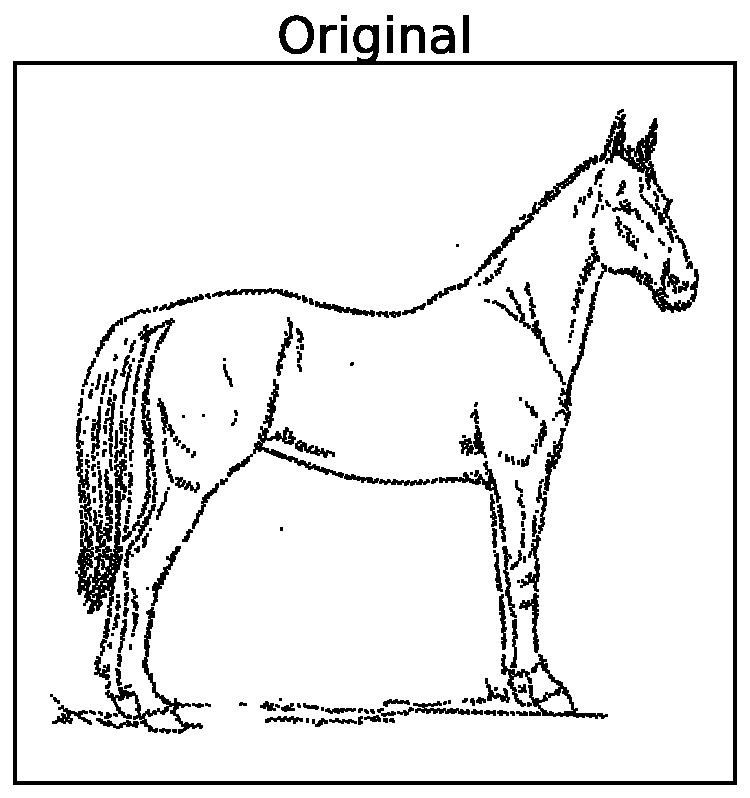
\includegraphics[width=\linewidth]{figures/OriginalHorse.pdf}
\end{subfigure}
%
\begin{subfigure}{.32\textwidth}
    \centering
    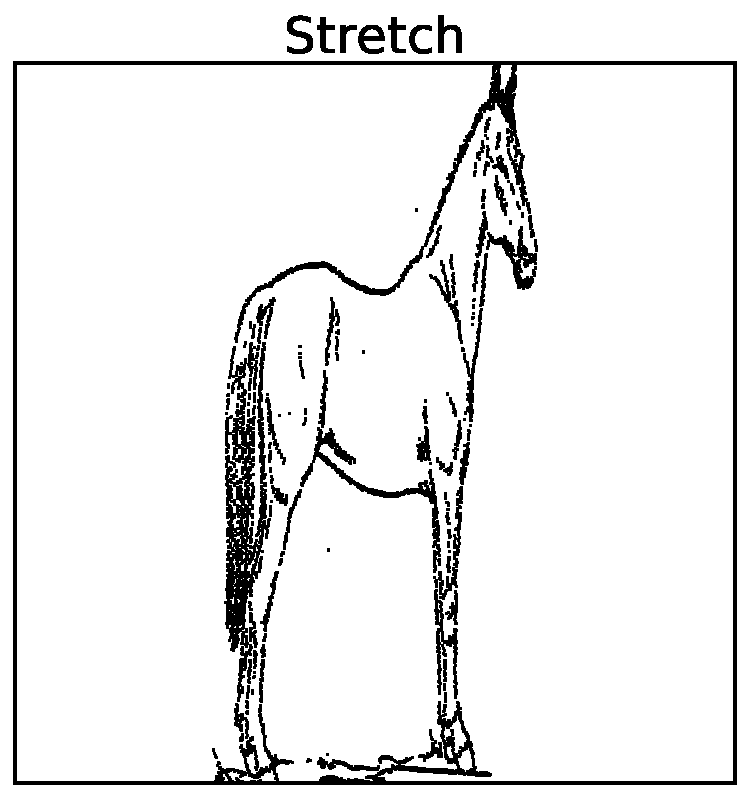
\includegraphics[width=\linewidth]{figures/StretchHorse.pdf}
\end{subfigure}
%
\begin{subfigure}{.32\textwidth}
    \centering
    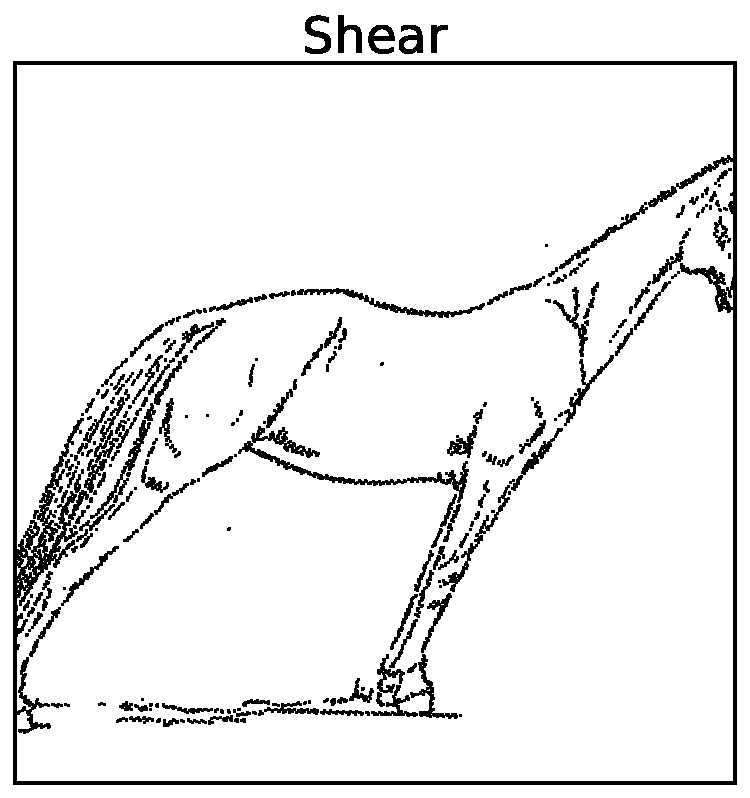
\includegraphics[width=\linewidth]{figures/ShearHorse.pdf}
\end{subfigure}
\\
\begin{subfigure}{.32\textwidth}
    \centering
    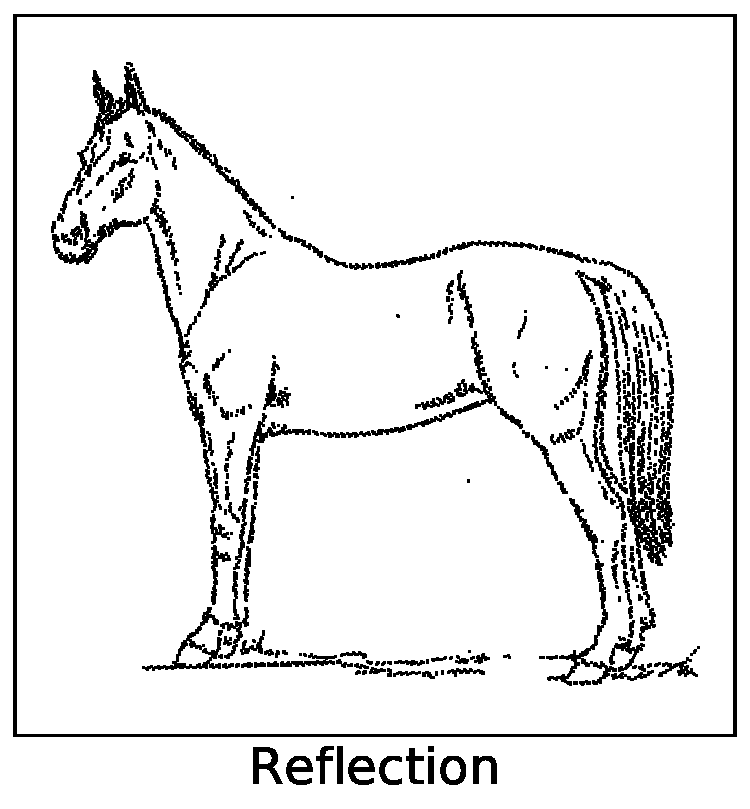
\includegraphics[width=\linewidth]{figures/ReflectionHorse.pdf}
\end{subfigure}
%
\begin{subfigure}{.32\textwidth}
    \centering
    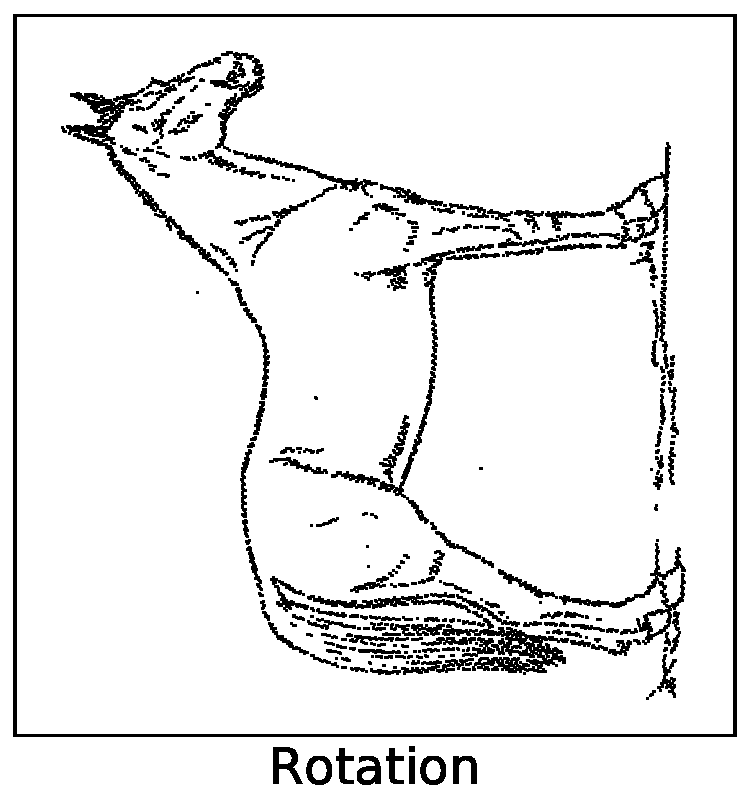
\includegraphics[width=\linewidth]{figures/RotationHorse.pdf}
\end{subfigure}
%
\begin{subfigure}{.32\textwidth}
    \centering
    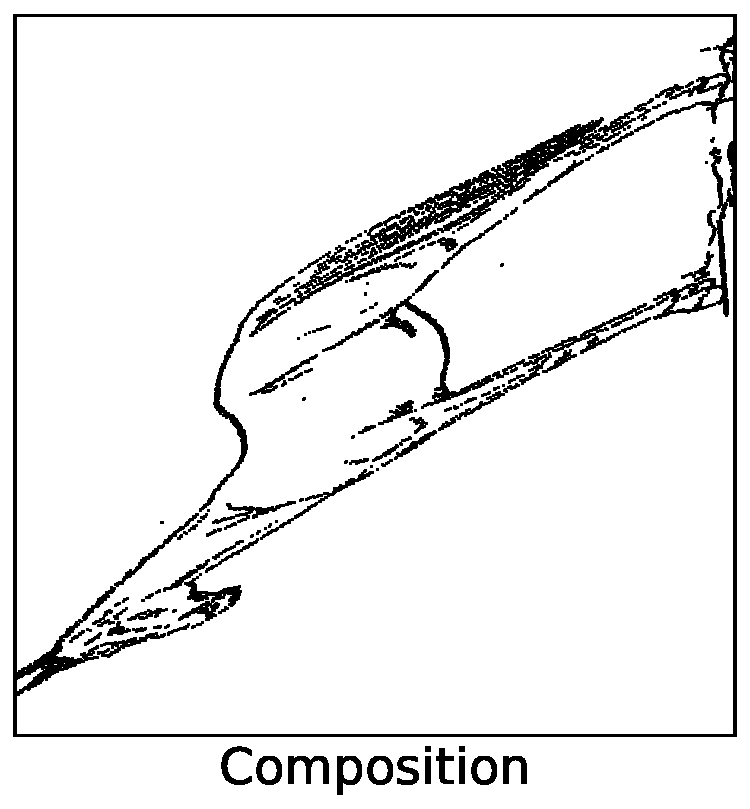
\includegraphics[width=\linewidth]{figures/CompositionHorse.pdf}
\end{subfigure}
\caption{The points stored in \texttt{horse.npy} under various linear transformations.}
\label{fig:linearly-transformed-horses}
\end{figure}


\begin{problem} % Implement linear transformations.
Write a function for each of the linear transformations listed above.
Each function should accept an array to transform and the scalars that define the transformation ($a$ and $b$ for stretch, shear, and reflection, and $\theta$ for rotation).
Construct the transformation matrix and left multiply it with the input array.
Return the transformed array.

To test your functions, consider writing a separate function that plots two arrays (the original and the transformed) for a side-by-side comparison.
\label{prob:implement-linear-transformations}
\end{problem}

\begin{info} % Look ahead to the QR decomposition.
Reflections and rotations are two ways to implement the QR Decomposition, an important matrix factorization which we will implement in a future lab. % In the next lab.
\end{info}

\subsection*{Compositions of Linear Transformations} % ------------------------

Let $V$, $W$, and $Z$ be finite-dimensional vector spaces.
If $L:V\rightarrow W$ and $K:W\rightarrow Z$ are linear transformations with transformation matrices $A$ and $B$, respectively, then the \emph{composition} $KL:V\rightarrow Z$ is also a linear transformation, and its transformation matrix is the matrix product $BA$.

For example, if $S$ is a matrix representing a shear and $R$ is a matrix representing a rotation, then $RS$ represents a shear followed by a rotation.
In fact, any linear transformation $L:\mathbb{R}^2 \rightarrow\mathbb{R}^2$ is a composition of the four transformations discussed above.
Figure \ref{fig:linearly-transformed-horses} displays the composition of all four previous transformations, applied in order (stretch, shear, reflection, then rotation).

\section*{Affine Transformations} % ===========================================

All linear transformations map the origin to itself.
An \emph{affine transformation} is a mapping between vector spaces that preserves the relationships between points and lines, but that may not preserve the origin.
Every affine transformation $T$ can be represented by a matrix $A$ and a vector $\b$.
To apply $T$ to a vector $x$, we calculate $A\x + \b$.
If $\b = \0$ then the transformation is linear, and if $A = I$ but $\b\neq\0$ then it is called a \emph{translation}.

For example, if $T$ is the translation with $\mathbf{b} = \left[\frac{3}{4}, \frac{1}{2}\right]\trp$, then applying $T$ to an image will shift it right by $\frac{3}{4}$ and up by $\frac{1}{2}$.
This translation is illustrated below.

\begin{figure}[H] % Generated with translated_horse() in plots.py.
\captionsetup[subfigure]{justification=centering}
\centering
\begin{subfigure}{.32\textwidth}
    \centering
    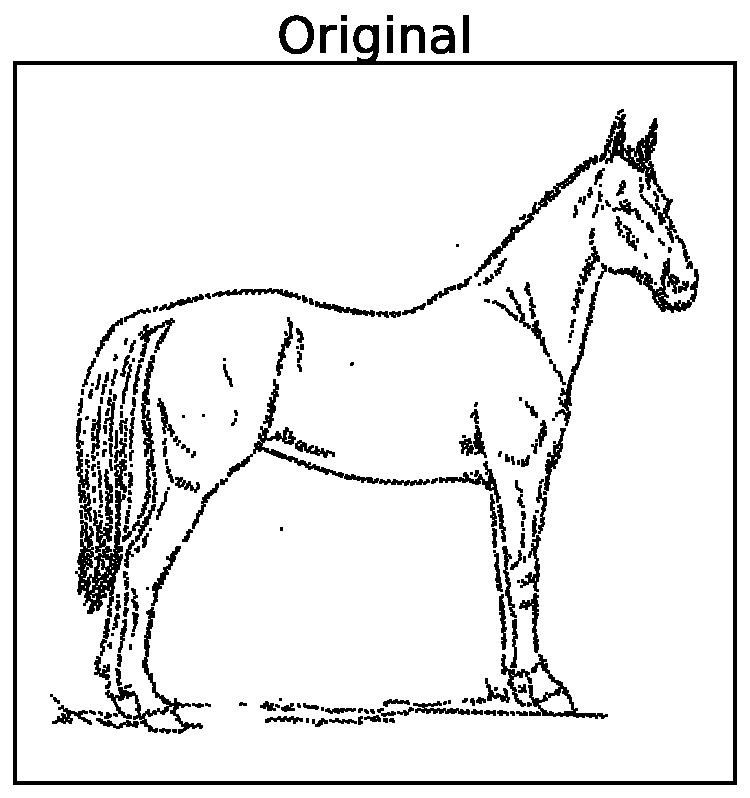
\includegraphics[width=\linewidth]{figures/OriginalHorse.pdf}
\end{subfigure}%
\begin{subfigure}{.32\textwidth}
    \centering
    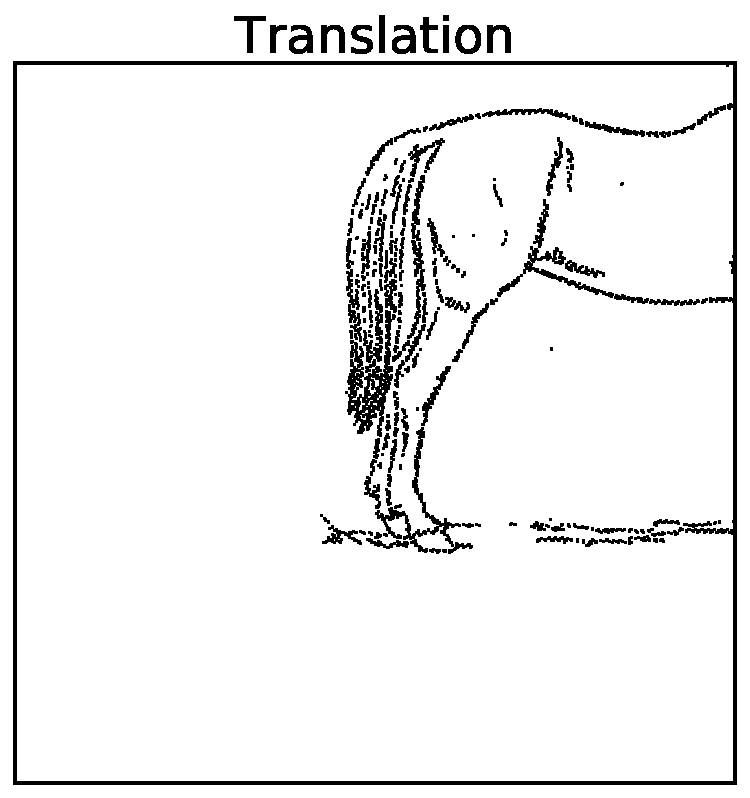
\includegraphics[width=\linewidth]{figures/TranslationHorse.pdf}
\end{subfigure}
\end{figure}

Affine transformations include all compositions of stretches, shears, rotations, reflections, and translations.
For example, if $S$ represents a shear and $R$ a rotation, and if $\b$ is a vector, then $RS\x + \b$ shears, then rotates, then translates $\x$.

\subsection*{Modeling Motion with Affine Transformations} % -------------------

Affine transformations can be used to model particle motion, such as a planet rotating around the sun.
Let the sun be the origin, the planet's location at time $t$ be given by the vector $\p(t)$, and suppose the planet has angular momentum $\omega$ (a measure of how fast the planet goes around the sun).
To find the planet's position at time $t$ given the planet's initial position $\p(0)$, rotate the vector $\p(0)$ around the origin by $t\omega$ radians.
Thus if $R(\theta)$ is the matrix representation of the linear transformation that rotates a vector around the origin by $\theta$ radians, then \[\p(t) = R(t\omega)\p(0).\]

Composing the rotation with a translation shifts the center of rotation away from the origin, yielding more complicated motion.

\begin{problem} % Moon orbiting the earth orbiting the sun.
The moon circles the earth while the earth orbits the sun.
Assuming circular orbits, we can compute the trajectories of both the earth and the moon using only linear and affine transformations.

Assume an orientation where both the earth and moon travel counterclockwise, with the sun at the origin.
Let $\p_e(t)$ and $\p_m(t)$ be the positions of the earth and the moon at time $t$, and let $\omega_e$ and $\omega_m$ be each celestial body's angular momentum.

\begin{enumerate}
\item Compute $\p_e(t)$ by rotating the initial vector $\p_e(0)$ counterclockwise about the origin by $t\omega_e$ radians.
\item Calculate the position of the moon relative to the earth at time $t$ by rotating the vector $\p_m(0) - \p_e(0)$ counterclockwise about the origin by $t\omega_m$ radians.
\item To compute $\p_m(t)$, translate the vector resulting from the previous step by $\p_e(t)$.
\end{enumerate}

Write a function that accepts a final time $T$ and the angular momenta $\omega_e$ and $\omega_m$.
Assuming initial positions $\p_e(0) = (10,0)$ and $\p_m(0) = (11,0)$, plot $\p_e(t)$ and $\p_m(t)$ over the time interval $t \in [0, T]$.

The moon travels around the earth approximately 13 times every year.
With $T = \frac{3\pi}{2}$, $\omega_e = 1$, and $\omega_m = 13$, your plot should resemble the following figure.
\\
\begin{figure}[H]
    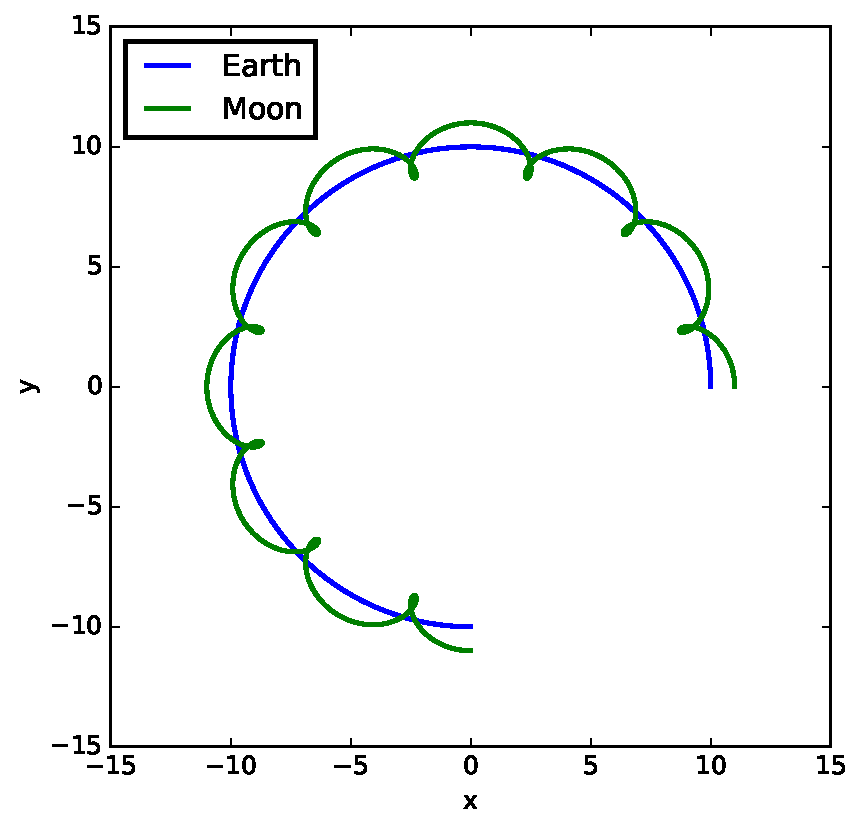
\includegraphics[width=.7\textwidth]{figures/SolarSystem.pdf}
\end{figure}

\label{prob:solar-system-trajectories}
\end{problem}

\section*{Timing Matrix Operations} % =========================================

% TODO: Transition sentence.

\subsection*{Timing Code} % ---------------------------------------------------

The \li{time} module in the standard library include functions for dealing with time.
The module's \li{time()} function measures the number of seconds from a fixed starting point, called ``the Epoch'' (January 1, 1970 for Unix machines).

\begin{lstlisting}
>>> import time
>>> time.time()
1466609325.819298
\end{lstlisting}

The \li{time()} function\footnote{The \li{clock()} function is similar to \li{time()}, but it records more precision on Windows machines.} is useful for measuring how long it takes for code to run: record the time just before and just after the code in question, then subtract the first measurement from the second to get the number of seconds that have passed.

\begin{lstlisting}
>>> def time_for_loop(iters):
...     """Time how long it takes to go through 'iters' iterations of nothing."""
...     start = time.time()         # Clock the starting time.
...     for _ in range(int(iters)):
...         pass
...     end = time.time()           # Clock the ending time.
...     return end - start          # Report the difference.
...
>>> time_for_loop(1e5)              # 1e5 = 100000.
0.007936954498291016
>>> time_for_loop(1e7)              # 1e7 = 10000000.
0.8008430004119873
\end{lstlisting}

The standard library's \li{timeit} module is built specifically to time code and has more sophisticated tools than the \li{time} module.
The \li{timeit()} function accepts a function handle (the name of the function to run) and the number of times to run it.
Additionally, in IPython the quick command \li{\%timeit} uses \li{timeit.timeit()} to quickly time a single line of code.

\begin{lstlisting}
In [1]: import timeit
In [2]: def for_loop():
   ...:     """Go through 1e7 iterations of nothing."""
   ...:     for _ in range(int(1e7)):
   ...:         pass

In [3]: timeit.timeit(for_loop, number=5) / 5.
Out[3]: 0.8081045627593995

In [4]: %timeit for_loop()
1 loop, best of 3: 801 ms per loop
\end{lstlisting}

\newpage

\subsection*{Timing an Algorithm} % -------------------------------------------

Most algorithms have at least one input that dictates the size of the problem to be solved.
For example, the following functions take in a single integer $n$ and produce a random vector of length $n$ as a list or a random $n\times n$ matrix as a list of lists.

\begin{lstlisting}
from random import random
def random_vector(n):       # Equivalent to np.random.random(n).tolist()
    """Generate a random vector of length n as a list."""
    return [random() for i in xrange(n)]

def random_matrix(n):       # Equivalent to np.random.random((n,n)).tolist()
    """Generate a random nxn matrix as a list of lists."""
    return [[random() for j in xrange(n)] for i in xrange(n)]
\end{lstlisting}

Executing \li{random_vector(n)} calls \li{random()} $n$ times, so doubling $n$ should about double the amount of time \li{random_vector(n)} takes to execute.
By contrast, executing \li{random_matrix(n)} calls \li{random()} $n^2$ times ($n$ times per row with $n$ rows).
Therefore doubling $n$ will likely more than double the amount of time \li{random_matrix(n)} takes to execute, especially if $n$ is large.

To visualize this phenomenon, we time \li{random_matrix()} for $n = 2^1,\ 2^2,\ \ldots,\ 2^{12}$ and plot $n$ against the execution time.
The result is displayed below on the left.% in Figure \ref{fig:matrix_time_result1}.

\begin{lstlisting}
>>> domain = 2**np.arange(1,13)
>>> times = []
>>> for n in domain:
...     start = time.time()
...     random_matrix(n)
...     times.append(time.time() - start)
...
>>> plt.plot(domain, times, 'g.-', linewidth=2, markersize=15)
>>> plt.xlabel("n", fontsize=14)
>>> plt.ylabel("Seconds", fontsize=14)
>>> plt.show()
\end{lstlisting}

\begin{figure}[H] % Generated with timing_demo() in plots.py.
\captionsetup[subfigure]{justification=centering}
\centering
\begin{subfigure}{.5\textwidth}
    \centering
    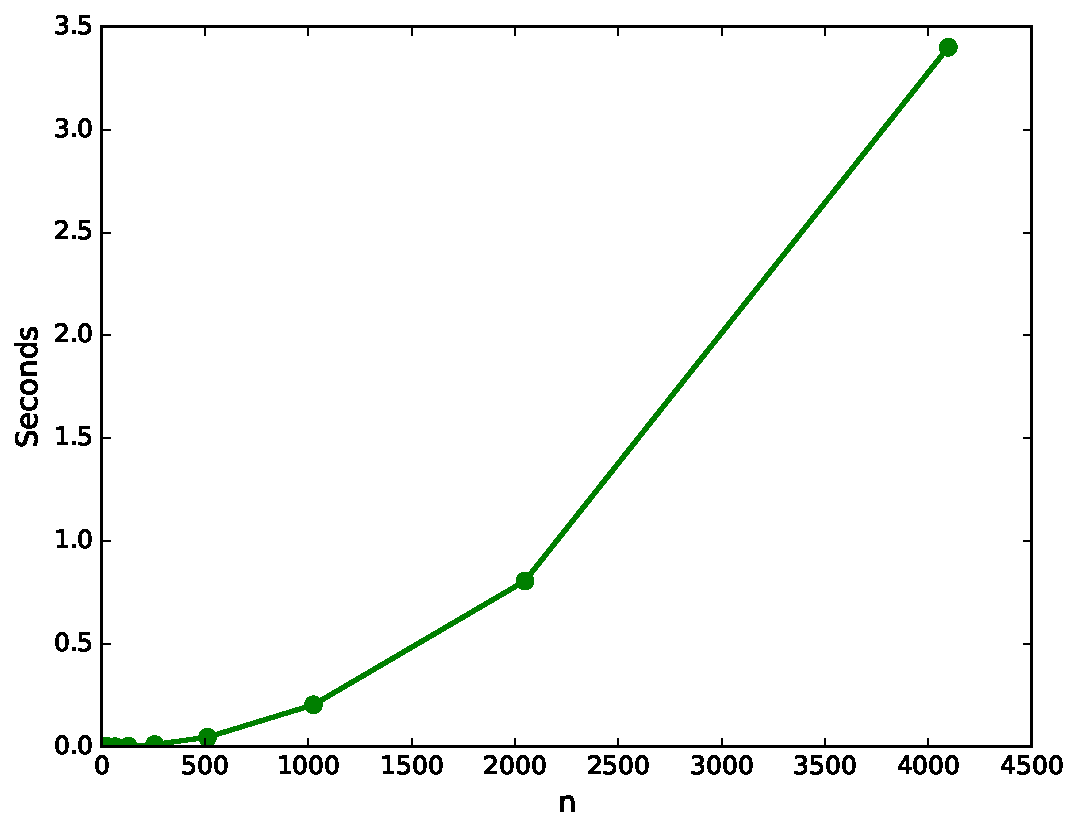
\includegraphics[width=\linewidth]{figures/time_random_matrix1.pdf}
    % \label{fig:matrix_time_result1}
\end{subfigure}%
\begin{subfigure}{.5\textwidth}
    \centering
    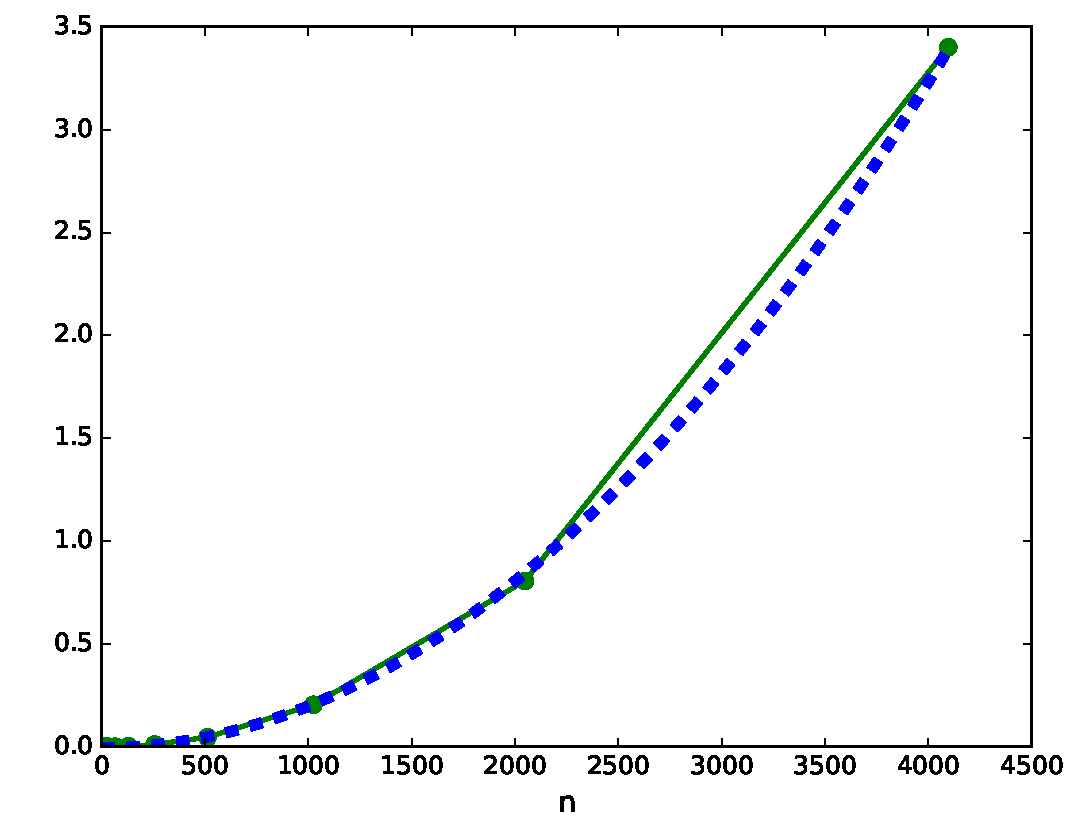
\includegraphics[width=\linewidth]{figures/time_random_matrix2.pdf}
\end{subfigure}
\end{figure}

The figure on the left shows that the execution time for \li{random_matrix(n)} increases quadratically in $n$.
In fact, the blue dotted line in the figure on the right is the parabola $y = an^2$, which fits nicely over the timed observations. Here $a$ is a small constant, but it is much less significant than the exponent on the $n$---we can leave it off altogether and write \li{random_matrix(n)} $\sim n^2$.%\footnote{In precise mathematical terms, we might write \li{random_matrix(n)} $\in O(n^2)$. See Volume II for more details on Big-O notation.}

% TODO: More explanation here? Reference to Vol II?

\begin{problem} % Time Matrix-Vector and Matrix-Matrix Multiplication.
Let $A$ be an $m \times n$ matrix with entries $a_{ij}$, $\x$ be an $n \times 1$ vector with entries $x_k$, and $B$ be an $n \times p$ matrix with entries $b_{ij}$.
%
% \begin{align*}
% A = \left[\begin{array}{cccc}
% a_{11} & a_{12} & \cdots & a_{1n} \\
% a_{21} & a_{22} & \cdots & a_{2n} \\
% \vdots & \vdots & \ddots & \vdots \\
% a_{m1} & a_{m2} & \cdots & a_{mn}
% \end{array}\right]
% &&
% \x = \left[\begin{array}{c}
% x_1 \\ x_2 \\ \vdots \\ x_n
% \end{array}\right]
% &&
% B = \left[\begin{array}{cccc}
% b_{11} & b_{12} & \cdots & b_{1p} \\
% b_{21} & b_{22} & \cdots & b_{2p} \\
% \vdots & \vdots & \ddots & \vdots \\
% b_{n1} & b_{n2} & \cdots & b_{np}
% \end{array}\right]
% \end{align*}

The matrix-vector product $A\x = \y$ is a new $m \times 1$ vector and the matrix-matrix product $AB = C$ is a new $m \times p$ matrix.
The entries $y_i$ of $\y$ and $c_{ij}$ of $C$ are determined by the following formulas:
%
\begin{align*}
y_i = \sum_{k=1}^n a_{ik}x_k%,\qquad i = 1,\ 2,\ \ldots,\ m.
&&
c_{ij} = \sum_{k=1}^n a_{ik}b_{kj}%,\quad i = 1,\, 2,\, \ldots,\ m, \quad j = 1,\, 2\, \ldots,\ l.
\end{align*}

Below, we implement these multiplication formulas without using NumPy.

\begin{lstlisting}
def matrix_vector_product(A, x):    # Equivalent to np.dot(A,x).tolist()
    """Compute the matrix-vector product Ax as a list."""
    m, n = len(A), len(x)
    return [sum([A[i][k] * x[k] for k in range(n)]) for i in range(m)]

def matrix_matrix_product(A, B):    # Equivalent to np.dot(A,B).tolist()
    """Compute the matrix-matrix product AB as a list of lists."""
    m, n, p = len(A), len(B), len(B[0])
    return [[sum([A[i][k] * B[k][j] for k in range(n)])
                                    for j in range(p) ]
                                    for i in range(m) ]
\end{lstlisting}

Use \li{time.time()}, \li{timeit.timeit()}, or \li{\%timeit} to time each of these functions with increasingly large inputs.
Generate the inputs $A$, $\x$, and $B$ with \li{random_matrix()} and \li{random_vector()} (so each input will be $n \times n$ or $n \times 1$).
Only time the multiplication functions, not the generating functions.

Report your findings in a single figure with two subplots: one with matrix-vector times, and one with matrix-matrix times.
Choose a domain for $n$ so that your figure accurately describes the growth, but avoid values of $n$ that lead to execution times of more than 1 minute.
Your figure should resemble the following plots.

\begin{figure}[H] % Generated with prob1_solution() in plots.py.
\captionsetup[subfigure]{justification=centering}
\centering
\begin{subfigure}{.5\textwidth}
    \centering
    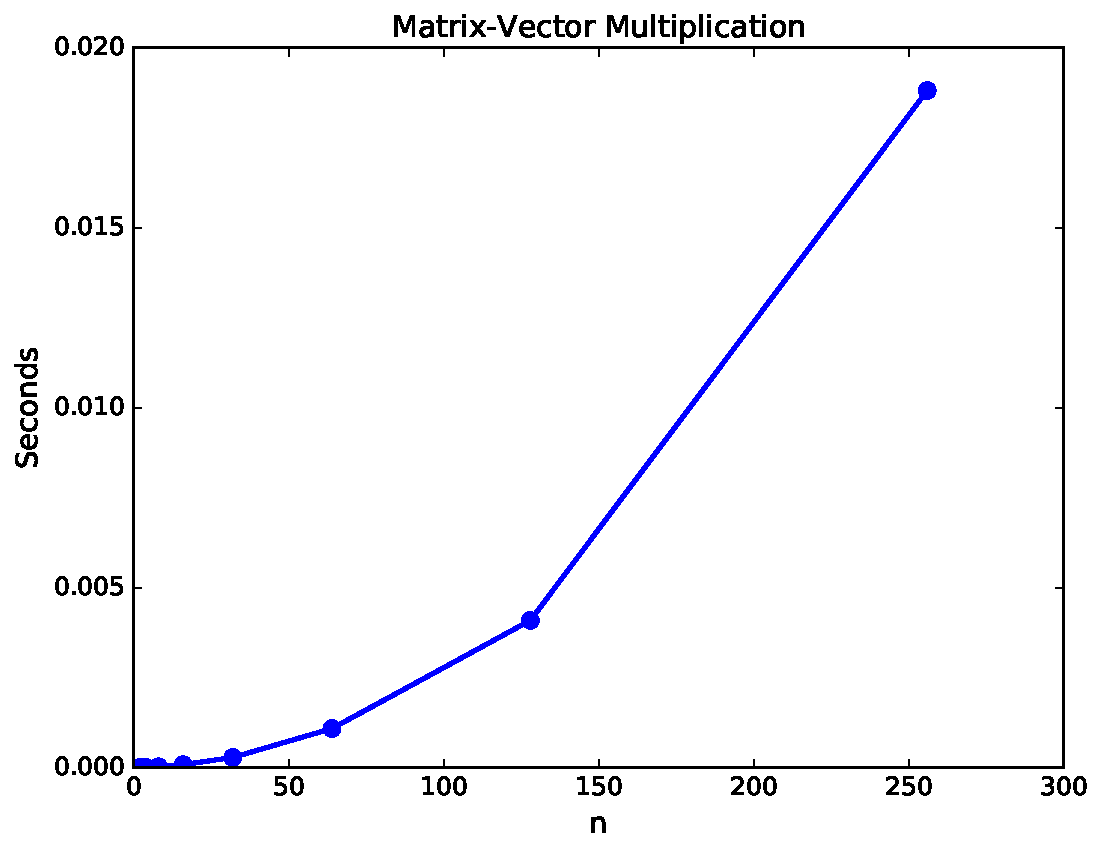
\includegraphics[width=\linewidth]{figures/matrixVectorMultiplication.pdf}
\end{subfigure}%
\begin{subfigure}{.474\textwidth}
    \centering
    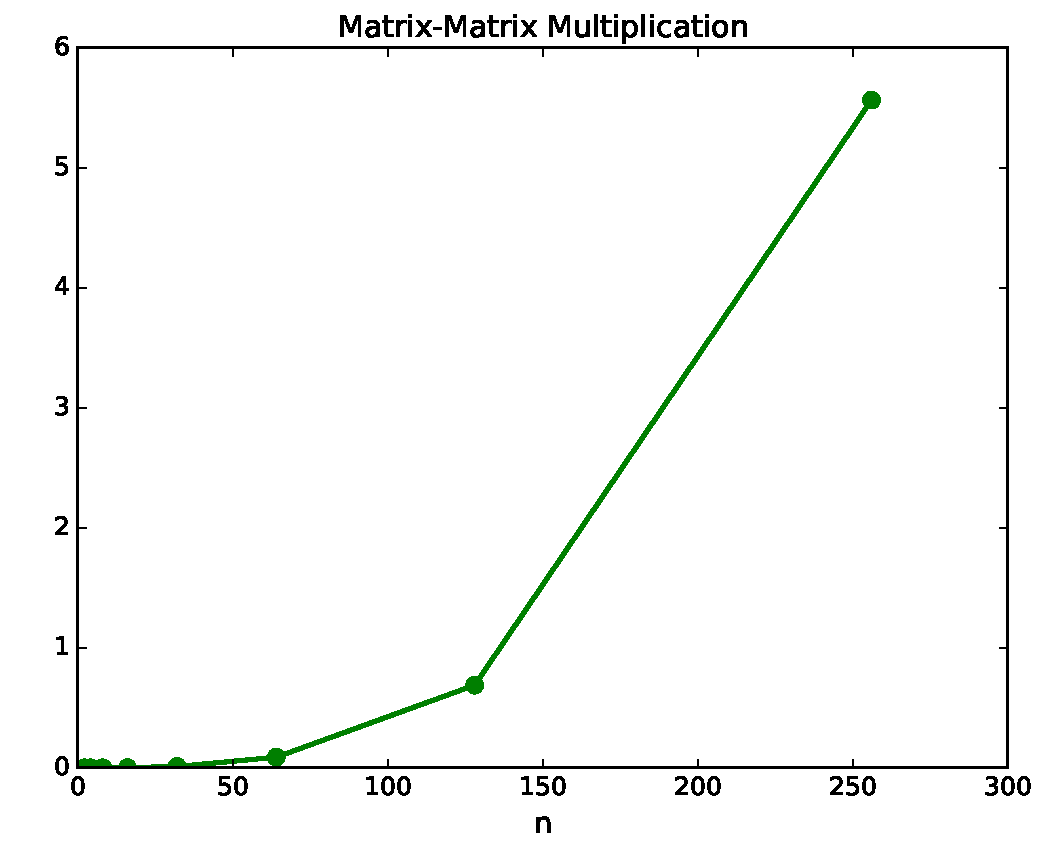
\includegraphics[width=\linewidth]{figures/matrixMatrixMultiplication.pdf}
\end{subfigure}
\end{figure}

\label{prob:matrix-multiplication-timing}
\end{problem}

\subsection*{Logarithmic Plots} % ---------------------------------------------

The two plots from Problem \ref{prob:matrix-multiplication-timing} look similar, but the actual execution times differ greatly.
To adequately compare the two, we need to view the results differently.

A \emph{logarithmic plot} uses a logarithmic scale---with values that increase exponentially, such as $10^1,\ 10^2,\ 10^3,\ \ldots$---on one or both of its axes.
The three kinds of log plots are listed below.

\begin{itemize}
\item \textbf{log-lin}: the $x$-axis uses a logarithmic scale but the $y$-axis uses a linear scale.\\
Use \li{plt.semilogx()} instead of \li{plt.plot()}.
\item \textbf{lin-log}: the $x$-axis is uses a linear scale but the $y$-axis uses a log scale.\\
Use \li{plt.semilogy()} instead of \li{plt.plot()}.
\item \textbf{log-log}: both the $x$ and $y$-axis use a logarithmic scale.\\
Use \li{plt.loglog()} instead of \li{plt.plot()}.
\end{itemize}

Since the domain $n = 2^1,\ 2^2,\ \ldots$ is a logarithmic scale and the execution times increase quadratically, we visualize the results of the previous problem with a log-log plot.
The default base for the logarithmic scales on logarithmic plots in Matplotlib is $10$.
To change the base to $2$ on each axis, specify the keyword arguments \li{basex=2} and \li{basey=2}.

Suppose the domain of $n$ values are stored in \li{domain} and the corresponding execution times for \li{matrix_vector_product()} and \li{matrix_matrix_product()} are stored in \li{vector_times} and \li{matrix_times}, respectively.
The following code produces Figure \ref{fig:loglogdemo}.

\begin{lstlisting}
>>> plt.subplot(121)        # Plot both curves on a lin-lin plot.
>>> plt.plot(domain, vector_times, 'b.-', lw=2, ms=15, label="Matrix-Vector")
>>> plt.plot(domain, matrix_times, 'g.-', lw=2, ms=15, label="Matrix-Matrix")
>>> plt.legend(loc="upper left")

>>> plot.subplot(122)       # Plot both curves on a base 2 log-log plot.
>>> plt.loglog(domain, vector_times, 'b.-', basex=2, basey=2, lw=2, ms=15)
>>> plt.loglog(domain, matrix_times, 'g.-', basex=2, basey=2, lw=2, ms=15)
>>> plt.show()
\end{lstlisting}

\begin{figure}[H] % Generated with loglog_demo() in plots.py.
\captionsetup[subfigure]{justification=centering}
\centering
\begin{subfigure}{.5\textwidth}
    \centering
    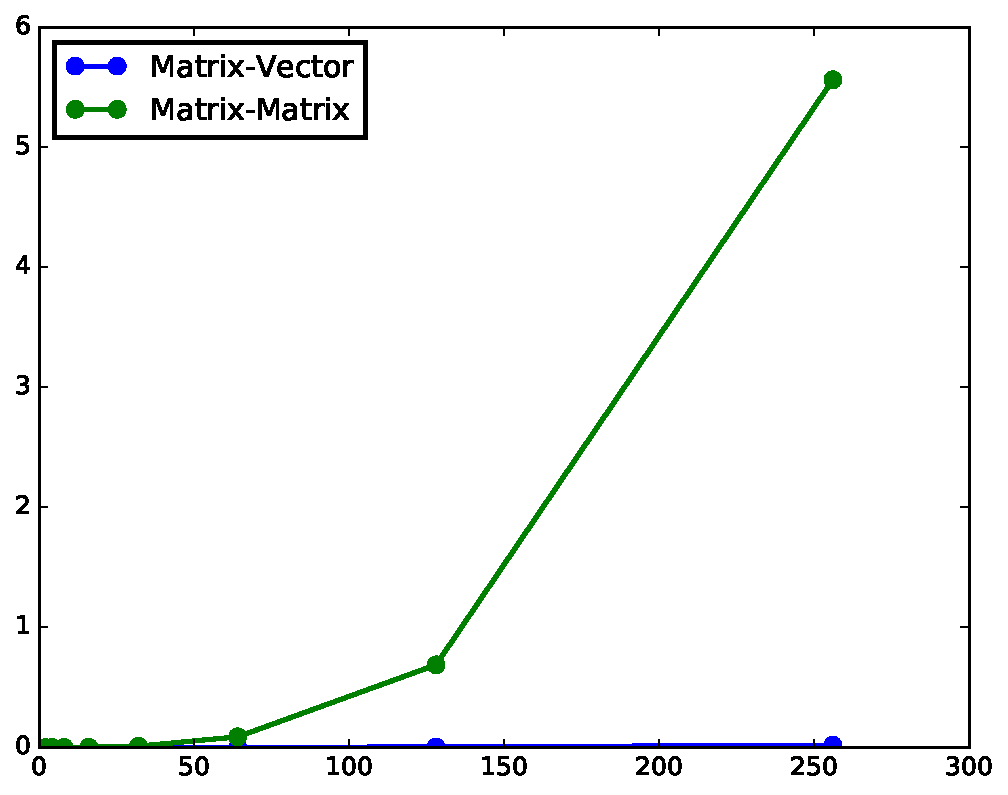
\includegraphics[width=\linewidth]{figures/loglogDemoBad.pdf}
\end{subfigure}%
\begin{subfigure}{.5\textwidth}
    \centering
    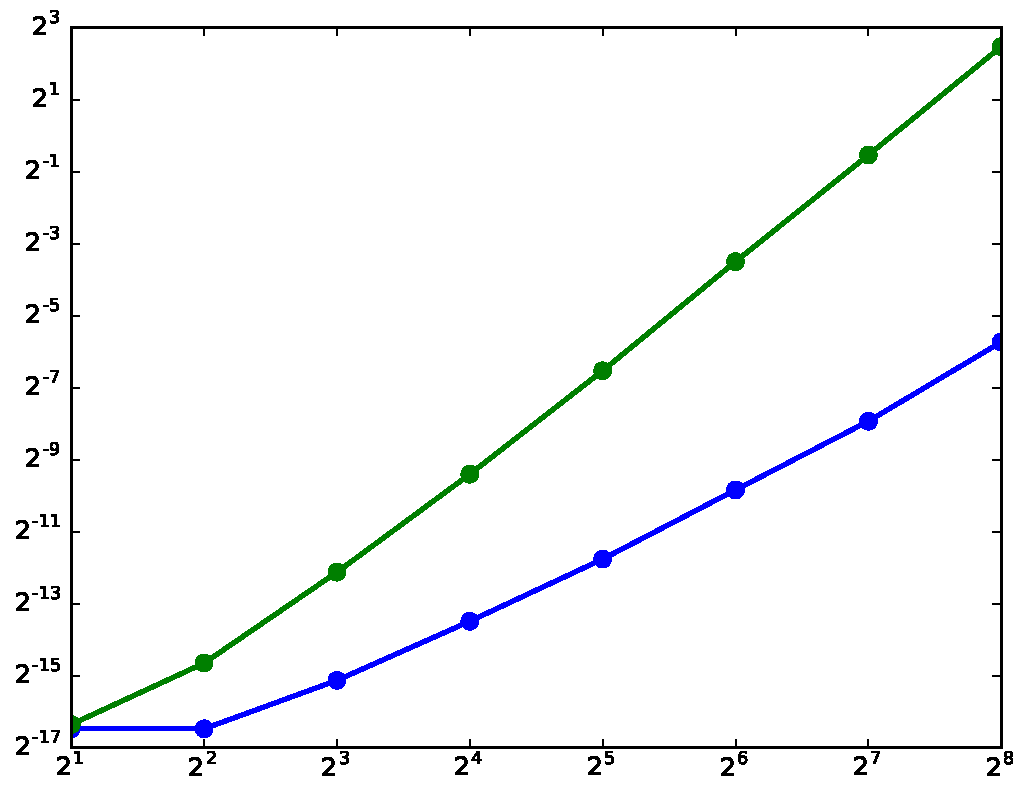
\includegraphics[width=\linewidth]{figures/loglogDemoGood.pdf}
\end{subfigure}
\caption{ }
\label{fig:loglogdemo}
\end{figure}

In the log-log plot, the slope of the \li{matrix_matrix_product()} line is about $3$ and the slope of the \li{matrix_vector_product()} line is about $2$.
This reflects the fact that matrix-matrix multiplication (which uses 3 \li{for} loops) is $\sim n^3$, while matrix-vector multiplication (which only has 2 loops) is only $\sim n^2$.

\begin{problem} % Why NumPy ROCKS.
NumPy is built specifically for fast numerical computations.
Repeat the experiment of Problem \ref{prob:matrix-multiplication-timing}, timing the following operations:
%
\begin{itemize}
\item matrix-vector multiplication with \li{matrix_vector_product()}.
\item matrix-matrix multiplication with \li{matrix_matrix_product()}.
\item matrix-vector multiplication with \li{np.dot()}.
\item matrix-matrix multiplication with \li{np.dot()}.
\end{itemize}

Create a single figure with two subplots: one with all four sets of execution times on a regular linear scale, and one with all four sets of execution times on a log-log scale.
Compare your results to Figure \ref{fig:loglogdemo}.
\label{prob:numpy-is-awesome}
\end{problem}

% TODO: Reword this note. What figure should be included?

\begin{info} % Note about Caching.
Problem \ref{prob:numpy-is-awesome} shows that \textbf{matrix  operations are significantly faster in NumPy than in plain Python}.
Matrix-matrix multiplication grows cubically regardless of the implementation; however, with lists the times grows at a rate of $an^3$ while with NumPy the times grow at a rate of $bn^3$, where $a$ is much larger than $b$.
% Since the exponent on the $n$ is the same in both cases, the disparity between the coefficients makes a significant impact.
% Iterating through loops is very expensive.
% NumPy also uses loops, but it uses C loops instead of Python loops.

% However, the execution times for matrix multiplication with NumPy seem to increase somewhat inconsistently.
% The fastest levels of computer memory can only handle so much information before it has to turn over to the next level of computer memory that is harder and slower to access.
% NumPy operations are optimized for computer hardware.
% Below, we plot execution times for vector-vector addition with NumPy.
% The spikes in the plot indicate the times that the array no longer fits in the current level of memory
%
% \begin{figure}[H]
% 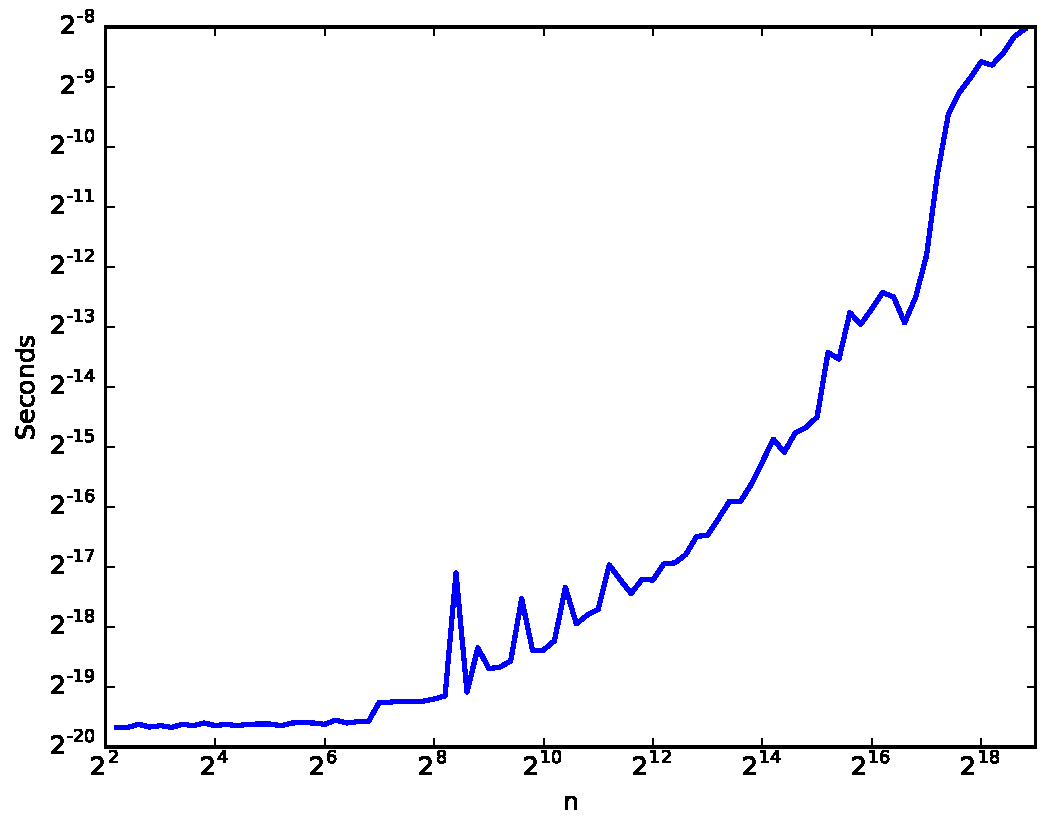
\includegraphics[width=.5\textwidth]{figures/cachingDemo.pdf}
% \end{figure}
\end{info}

\newpage

\section*{Additional Material} % ==============================================

\subsection*{Image Transformation as a Class} % -------------------------------

Consider organizing the functions from Problem \ref{prob:implement-linear-transformations} into a class.
The constructor might accept an array or the name of a file containing an array.
This structure would makes it easy to do several linear or affine transformations in sequence.

\begin{lstlisting}
>>> horse = ImageTransformer("horse.npy")
>>> horse.stretch(.5, 1.2)
>>> horse.shear(.5, 0)
>>> horse.relect(0, 1)
>>> horse.rotate(np.pi/2.)
>>> horse.translate(.75, .5)
>>> horse.display()
\end{lstlisting}

\subsection*{Animating Parametrizations} % ------------------------------------

The plot in Problem \ref{prob:solar-system-trajectories} fails to fully convey the system's evolution over time because time itself is not part of the plot.
The following function creates a simple Matplotlib animation for the earth and moon trajectories.

\begin{lstlisting}
from matplotlib import animation

def solar_system_animation(earth, moon):
    """Animate the moon orbiting the earth and the earth orbiting the sun.
    Inputs:
        earth ((2,N) ndarray): The earth's postion with x-coordinates on the
            first row and y coordinates on the second row.
        moon ((2,N) ndarray): The moon's postion with x-coordinates on the
            first row and y coordinates on the second row.
    """
    animation_fig = plt.figure()                    # Make a new figure.
    plt.axis([-15,15,-15,15])                       # Set the window limits.
    plt.gca().set_aspect("equal")                   # Make the window square.

    earth_dot,  = plt.plot([],[], 'bo', ms=10)      # Blue dot for the earth.
    earth_path, = plt.plot([],[], 'b-')             # Blue line for the earth.
    moon_dot,   = plt.plot([],[], 'go', ms=5)       # Green dot for the moon.
    moon_path,  = plt.plot([],[], 'g-')             # Green line for the moon.
    plt.plot([0],[0],'y*', ms=30)                   # Yellow star for the sun.

    def animate(index):
        """Update the four earth and moon plots."""
        earth_dot.set_data(earth[0,index], earth[1,index])
        earth_path.set_data(earth[0,:index], earth[1,:index])
        moon_dot.set_data(moon[0,index], moon[1,index])
        moon_path.set_data(moon[0,:index], moon[1,:index])
        return earth_dot, earth_path, moon_dot, moon_path

    a = animation.FuncAnimation(animation_fig, animate,
                                frames=earth.shape[1], interval=25)
    plt.show()
\end{lstlisting}

See \url{http://matplotlib.org/1.5.1/examples/animation/index.html} for other examples of animations in Matplotlib.

\begin{comment} % TODO: Fix this.
\subsection*{Celestial Mechanics} % -------------------------------------------

In the early 1600s Johannes Kepler discovered that planets travel around the sun in elliptical orbits.
Simulating an elliptical orbit is more complicated than simulating a circular orbit because the speed and angular momentum of the celestial body are not constant in time.
However, with only 2 bodies (the earth and the sun), it is still fairly simple to completely describe the system for all time.
Once a third body (the moon) is introduced into the system, however, it becomes incredibly difficult to accurately describe the system.
% This phenomenon is referred to as the 3-body problem.
\end{comment}
